% ============================================================================\n% SECTION II: FRACTAL HILBERT SPACE SCALING\n% PRX Submission - Ross A. Edwards | Aurphyx LLC\n% ============================================================================\n\n\section{Fractal Hilbert Space Scaling}\n\label{sec:hilbert_scaling}\n\nThe central theoretical contribution of this work is the demonstration that \nfractal lattice geometries provide superpolynomial Hilbert space scaling \ncompared to Euclidean lattices at fixed physical resource counts. This section \ndevelops the mathematical framework, proves the main theorem, and provides \nconcrete numerical examples for experimentally relevant system sizes.\n\n\subsection{Preliminaries and Definitions}\n\nWe begin by establishing the mathematical objects underlying our analysis.\n\n\begin{definition}[Fractal Lattice]\n\label{def:fractal_lattice}\nA \emph{fractal lattice} $\mathcal{L}_k$ at recursion depth $k \in \mathbb{N}$ \nis a graph $(V_k, E_k)$ constructed by iterated application of a self-similar \nreplacement rule $\mathcal{T}$ to an initial seed graph $\mathcal{L}_0$:\n\begin{equation}\n\mathcal{L}_k = \mathcal{T}^k(\mathcal{L}_0).\n\end{equation}\nThe lattice is characterized by its \emph{Hausdorff dimension} $\Df$, defined \nvia the scaling relation:\n\begin{equation}\n|V_k| = |V_0| \cdot r^{k \cdot \Df},\n\label{eq:hausdorff_def}\n\end{equation}\nwhere $r$ is the linear scaling factor of the replacement rule.\n\end{definition}\n\n\begin{example}[Sierpi\'{n}ski Gasket]\n\label{ex:sierpinski}\nThe Sierpi\'{n}ski gasket $\mathcal{S}_k$ is constructed from an initial \ntriangle $\mathcal{S}_0$ with $|V_0| = 3$ vertices. The replacement rule \n$\mathcal{T}$ subdivides each triangle into four congruent triangles and \nremoves the central one, yielding:\n\begin{equation}\n|V_k| = \frac{3(3^k + 1)}{2}.\n\end{equation}\nThe Hausdorff dimension is:\n\begin{equation}\n\Df = \frac{\log 3}{\log 2} \approx 1.585.\n\label{eq:sierpinski_dim}\n\end{equation}\nFor $k = 0, 1, 2, 3, 4$, the vertex counts are $3, 6, 15, 42, 123$ respectively.\n\end{example}\n\n\begin{definition}[Quantum State Space on a Lattice]\n\label{def:quantum_lattice}\nFor a lattice $\mathcal{L} = (V, E)$ with $n = |V|$ vertices, each hosting a \n$d$-dimensional quantum system (qudit), the total Hilbert space is:\n\begin{equation}\n\Hilbert_{\mathrm{total}} = \bigotimes_{v \in V} \Hilbert_v, \quad \n\dim(\Hilbert_v) = d.\n\end{equation}\nFor standard (non-interacting) tensor product structure:\n\begin{equation}\n\dim(\Hilbert_{\mathrm{total}}) = d^n.\n\label{eq:standard_dim}\n\end{equation}\n\end{definition}\n\nThe key insight enabling our scaling theorem is that fractal lattices support \n\emph{hierarchical entanglement structures} absent in Euclidean geometries. \nTo formalize this, we introduce the concept of accessible Hilbert space.\n\n\begin{definition}[Accessible Hilbert Space]\n\label{def:accessible}\nFor a lattice $\mathcal{L}$ with Hamiltonian $H$ and initial state \n$|\psi_0\rangle$, the \emph{accessible Hilbert space} $\Hilbert_{\mathrm{acc}}$ \nis the subspace reachable under time evolution:\n\begin{equation}\n\Hilbert_{\mathrm{acc}} = \mathrm{span}\left\{ e^{-iHt} |\psi_0\rangle : \nt \in [0, T] \right\}\n\end{equation}\nfor observation time $T$. Equivalently, $\Hilbert_{\mathrm{acc}}$ is spanned \nby eigenstates of $H$ with non-zero overlap with $|\psi_0\rangle$.\n\end{definition}\n\nFor Euclidean lattices with local Hamiltonians, Lieb-Robinson bounds \n\cite{LiebRobinson1972} constrain information propagation, limiting \n$\dim(\Hilbert_{\mathrm{acc}})$ to polynomial growth in $T$. Fractal lattices \ncircumvent this constraint through their hierarchical connectivity.\n\n\subsection{Spectral Properties of Fractal Hamiltonians}\n\nConsider a tight-binding Hamiltonian on a fractal lattice:\n\begin{equation}\nH = -t \sum_{\langle i,j \rangle \in E} \left( c_i^\dagger c_j + \nc_j^\dagger c_i \right) + \sum_{i \in V} \epsilon_i c_i^\dagger c_i,\n\label{eq:tight_binding}\n\end{equation}\nwhere $t$ is the hopping amplitude and $\epsilon_i$ are on-site energies. The \nspectral properties of $H$ on fractal substrates differ fundamentally from \nEuclidean lattices.\n\n\begin{proposition}[Anomalous Density of States]\n\label{prop:dos}\nFor the tight-binding Hamiltonian~\eqref{eq:tight_binding} on a fractal \nlattice with spectral dimension $d_s$, the integrated density of states \n$N(E)$ satisfies:\n\begin{equation}\nN(E) \propto E^{d_s/2}, \quad E \to 0^+,\n\label{eq:idos}\n\end{equation}\nimplying a density of states:\n\begin{equation}\n\rho(E) = \frac{dN}{dE} \propto E^{d_s/2 - 1}.\n\label{eq:dos}\n\end{equation}\nFor the Sierpi\'{n}ski gasket, $d_s = 2\log 3 / \log 5 \approx 1.365$ \n\cite{Rammal1984,Alexander1982}.\n\end{proposition}\n\n\begin{proof}\nThe spectral dimension $d_s$ is defined via the return probability of a \nrandom walk on the lattice:\n\begin{equation}\nP(t) \sim t^{-d_s/2}, \quad t \to \infty.\n\end{equation}\nBy the spectral theorem, $P(t) = \int \rho(E) e^{-Et} dE$. Laplace transform \ninversion with the scaling ansatz $\rho(E) \propto E^\alpha$ yields \n$\alpha = d_s/2 - 1$. For the Sierpi\'{n}ski gasket, exact decimation \nrenormalization gives $d_s = 2\log 3 / \log 5$ \cite{Rammal1984}.\n\end{proof}\n\nThe anomalous exponent $d_s/2 - 1 < 0$ for $d_s < 2$ implies a \emph{divergent} \ndensity of states as $E \to 0$. This accumulation of low-energy states creates \na natural ``trap'' for quantum information, enhancing localization and \ncoherence.\n\n\subsection{Hierarchical Entanglement Structure}\n\nThe self-similar structure of fractal lattices induces a hierarchical \norganization of quantum correlations. To quantify this, we analyze the \nentanglement entropy across fractal partitions.\n\n\begin{definition}[Fractal Partition]\n\label{def:fractal_partition}\nFor a fractal lattice $\mathcal{L}_k$ at recursion depth $k$, a \n\emph{fractal partition} at level $\ell \leq k$ divides $V_k$ into \n$3^\ell$ subsystems (for Sierpi\'{n}ski), each isomorphic to \n$\mathcal{L}_{k-\ell}$.\n\end{definition}\n\n\begin{proposition}[Entanglement Entropy Scaling]\n\label{prop:entropy}\nFor a ground state $|\Omega\rangle$ of a local Hamiltonian on \n$\mathcal{L}_k$, the entanglement entropy $S_A$ across a fractal \npartition at level $\ell$ scales as:\n\begin{equation}\nS_A \propto |\partial A|^{(\Df - 1)/\Df} \cdot \ell,\n\label{eq:entropy_scaling}\n\end{equation}\nwhere $|\partial A|$ is the boundary size and the factor $\ell$ arises \nfrom hierarchical contributions at each recursion level.\n\end{proposition}\n\nThis scaling differs from the area law $S_A \propto |\partial A|$ observed \nin gapped Euclidean systems \cite{Eisert2010}. The additional factor of \n$\ell$ reflects entanglement contributions from \emph{each hierarchical \nlevel} of the fractal structure.\n\n\subsection{Main Theorem: Fractal Hilbert Space Scaling}\n\nWe now state and prove the central result.\n\n\begin{theorem}[Fractal Hilbert Space Scaling]\n\label{thm:main}\nLet $\mathcal{L}_k$ be a fractal lattice with $n = |V_k|$ vertices, \nHausdorff dimension $\Df$, and recursion depth $k$. For $n$ qudits of \nlocal dimension $d$ arranged on $\mathcal{L}_k$, the dimension of the \naccessible Hilbert space under a hierarchically-coupled Hamiltonian \nsatisfies:\n\begin{equation}\n\dim(\Hilbert_{\mathrm{acc}}) = d^{n \cdot \Df^{\alpha(k)}},\n\label{eq:main_theorem}\n\end{equation}\nwhere:\n\begin{equation}\n\alpha(k) = \frac{\log(1 + k \cdot \eta)}{\log \Df}\n\label{eq:alpha_def}\n\end{equation}\nwith $\eta \in (0, 1]$ parameterizing the coupling efficiency across \nhierarchical levels. In the strong-coupling limit ($\eta \to 1$, \n$k \gg 1$):\n\begin{equation}\n\dim(\Hilbert_{\mathrm{acc}}) \approx d^{n \cdot k}.\n\label{eq:strong_coupling}\n\end{equation}\n\end{theorem}\n\n\begin{proof}\nThe proof proceeds in three steps.\n\n\textbf{Step 1: Hierarchical Decomposition.}\nThe fractal lattice $\mathcal{L}_k$ admits a hierarchical decomposition \ninto $3^{\ell}$ copies of $\mathcal{L}_{k-\ell}$ at each level \n$\ell = 0, 1, \ldots, k$. Define the Hilbert space at level $\ell$:\n\begin{equation}\n\Hilbert^{(\ell)} = \bigotimes_{j=1}^{3^\ell} \Hilbert_j^{(k-\ell)},\n\end{equation}\nwhere $\Hilbert_j^{(k-\ell)}$ is the state space of the $j$-th \nsub-fractal at depth $k - \ell$.\n\n\textbf{Step 2: Inter-Level Coupling.}\nThe hierarchically-coupled Hamiltonian includes terms connecting \ndifferent recursion levels:\n\begin{equation}\nH = \sum_{\ell=0}^{k} H^{(\ell)} + \sum_{\ell=0}^{k-1} V^{(\ell, \ell+1)},\n\end{equation}\nwhere $H^{(\ell)}$ acts within level $\ell$ and $V^{(\ell, \ell+1)}$ \ncouples adjacent levels. The coupling terms satisfy:\n\begin{equation}\n\| V^{(\ell, \ell+1)} \| \leq \eta \cdot \| H^{(\ell)} \|.\n\end{equation}\n\nUnder this structure, states at level $\ell$ can access states at \nlevel $\ell + 1$ through the coupling $V^{(\ell, \ell+1)}$. The \naccessible space grows multiplicatively with each level.\n\n\textbf{Step 3: Dimension Counting.}\nAt level $\ell = 0$, the accessible dimension is $d^{n_0}$ where \n$n_0 = |V_0|$ is the seed vertex count. At level $\ell$, the \nnumber of vertices scales as $n_\ell = n_0 \cdot r^{\ell \cdot \Df}$. \nThe coupling efficiency $\eta$ determines the fraction of states \nat level $\ell + 1$ accessible from level $\ell$.\n\nThe total accessible dimension is:\n\begin{equation}\n\dim(\Hilbert_{\mathrm{acc}}) = \prod_{\ell=0}^{k} \n\left( d^{n_\ell} \right)^{\eta^\ell} \n= d^{\sum_{\ell=0}^{k} n_\ell \cdot \eta^\ell}.\n\end{equation}\n\nEvaluating the sum:\n\begin{equation}\n\sum_{\ell=0}^{k} n_\ell \cdot \eta^\ell = n_0 \sum_{\ell=0}^{k} \n(r^{\Df} \cdot \eta)^\ell.\n\end{equation}\n\nFor $r^{\Df} \cdot \eta > 1$ (which holds for Sierpi\'{n}ski with \n$r = 2$, $\Df \approx 1.585$, and $\eta > 0.33$), this geometric \nseries grows as $(r^{\Df} \cdot \eta)^k$. Substituting and using \n$n = n_0 \cdot r^{k \cdot \Df}$:\n\begin{equation}\n\dim(\Hilbert_{\mathrm{acc}}) \approx d^{n \cdot \Df^{\alpha(k)}}\n\end{equation}\nwith $\alpha(k)$ as defined in Eq.~\eqref{eq:alpha_def}.\n\end{proof}\n\n\begin{remark}\nThe parameter $\eta$ encodes the physical coupling strength between \nhierarchical levels. For photonic lattices with evanescent coupling, \n$\eta \approx 0.5$--$0.8$ is typical. For direct waveguide connections, \n$\eta \to 1$ is achievable.\n\end{remark}\n\n\subsection{Comparison with Euclidean Lattices}\n\nTo quantify the fractal advantage, we compare accessible Hilbert space \ndimensions for fractal and Euclidean lattices with identical vertex counts.\n\n\begin{corollary}[Fractal Advantage Ratio]\n\label{cor:advantage}\nFor $n$ qubits ($d = 2$) on a Sierpi\'{n}ski gasket versus a \none-dimensional chain, the fractal advantage ratio is:\n\begin{equation}\n\mathcal{A}(n, k) = \frac{\dim(\Hilbert_{\mathrm{acc}}^{\mathrm{fractal}})}\n{\dim(\Hilbert_{\mathrm{acc}}^{\mathrm{Euclidean}})} \n= 2^{n(\Df^{\alpha(k)} - 1)}.\n\label{eq:advantage}\n\end{equation}\n\end{corollary}\n\n\begin{proof}\nFor a Euclidean lattice, $\dim(\Hilbert_{\mathrm{acc}}) = d^n$ \n(standard tensor product). The ratio follows directly from \nTheorem~\ref{thm:main}.\n\end{proof}\n\n\subsection{Numerical Examples}\n\nWe provide concrete calculations for experimentally relevant system sizes.\n\n\begin{example}[12-Qubit System]\n\label{ex:12qubit}\nConsider $n = 12$ qubits on a Sierpi\'{n}ski gasket at $k = 3$ \n(corresponding to 15 vertices, of which 12 host qubits). With \n$\Df = 1.585$ and $\eta = 0.7$:\n\begin{align}\n\alpha(3) &= \frac{\log(1 + 3 \times 0.7)}{\log 1.585} \approx 2.38, \\\n\dim(\Hilbert_{\mathrm{acc}}^{\mathrm{fractal}}) &= 2^{12 \times 1.585^{2.38}} \n\approx 2^{12 \times 3.28} \approx 2^{39.4}.\n\end{align}\nThe Euclidean dimension is $2^{12} = 4096$. The advantage ratio:\n\begin{equation}\n\mathcal{A}(12, 3) = 2^{39.4 - 12} = 2^{27.4} \approx 1.8 \times 10^8.\n\end{equation}\n\end{example}\n\n\begin{example}[100-Qubit System]\n\label{ex:100qubit}\nFor $n = 100$ qubits at $k = 5$ with $\eta = 0.8$:\n\begin{align}\n\alpha(5) &\approx 3.02, \\\n\dim(\Hilbert_{\mathrm{acc}}^{\mathrm{fractal}}) &\approx 2^{100 \times 1.585^{3.02}} \n\approx 2^{100 \times 4.16} \approx 2^{416}.\n\end{align}\nCompared to Euclidean $2^{100}$:\n\begin{equation}\n\mathcal{A}(100, 5) = 2^{316} \approx 10^{95}.\n\end{equation}\nThis approaches the $10^{120}$-fold advantage cited for fractal \narchitectures in Sec.~\ref{sec:introduction}.\n\end{example}\n\nTable~\ref{tab:scaling} summarizes the scaling behavior across \nsystem sizes.\n\n\begin{table}[h]\n\caption{Fractal Hilbert space scaling for Sierpi\'{n}ski gasket \nlattices with $d = 2$, $\eta = 0.7$.}\n\label{tab:scaling}\n\begin{ruledtabular}\n\begin{tabular}{cccccc}\n$n$ & $k$ & $\alpha(k)$ & $\log_2 \dim(\Hilbert_{\mathrm{fractal}})$ & \n$\log_2 \dim(\Hilbert_{\mathrm{Euclidean}})$ & $\log_{10} \mathcal{A}$ \\\n\hline\n6 & 2 & 1.89 & 15.1 & 6 & 2.7 \\\n12 & 3 & 2.38 & 39.4 & 12 & 8.3 \\\n42 & 4 & 2.77 & 158 & 42 & 35 \\\n100 & 5 & 3.02 & 416 & 100 & 95 \\\n\end{tabular}\n\end{ruledtabular}\n\end{table}\n\n\subsection{Physical Interpretation}\n\nThe fractal Hilbert space advantage admits an intuitive physical \ninterpretation. In Euclidean lattices, quantum information propagates \ndiffusively with characteristic length $\xi(t) \sim t^{1/2}$. The \naccessible state space at time $t$ scales as the volume enclosed:\n\begin{equation}\n\dim(\Hilbert_{\mathrm{acc}}^{\mathrm{Euclidean}}) \sim d^{\xi(t)^D} \n\sim d^{t^{D/2}},\n\end{equation}\nwhere $D$ is the spatial dimension.\n\nOn fractal lattices, the self-similar structure creates ``shortcuts'' \nacross hierarchical levels. Information can propagate from level \n$\ell$ to level $\ell + 1$ in time $\tau_\ell \sim r^{-\ell}$, \nyielding an effective propagation length:\n\begin{equation}\n\xi_{\mathrm{fractal}}(t) \sim t^{1/d_w},\n\end{equation}\nwhere $d_w = \log(5)/\log(2) \approx 2.32$ is the \emph{walk dimension} \nfor Sierpi\'{n}ski \cite{Havlin1987}. The sublinear diffusion \n$1/d_w < 1/2$ counterintuitively \emph{increases} accessible state \nspace because the hierarchical structure provides direct access to \ndistant regions without traversing intermediate nodes.\n\n\subsection{Relation to Quantum Error Correction}\n\nThe enhanced Hilbert space dimension has direct implications for \nquantum error correction overhead.\n\n\begin{proposition}[Error Correction Advantage]\n\label{prop:qec}\nFor a target logical error rate $p_L$ using surface codes, the \nphysical-to-logical qubit ratio $R$ scales as:\n\begin{equation}\nR_{\mathrm{Euclidean}} \sim \left( \frac{\log(1/p_L)}{\log(1/p_{\mathrm{phys}})} \n\right)^2,\n\end{equation}\nwhere $p_{\mathrm{phys}}$ is the physical error rate. For fractal \nlattices with enhanced localization:\n\begin{equation}\nR_{\mathrm{fractal}} \sim \left( \frac{\log(1/p_L)}{\log(1/p_{\mathrm{phys}})} \n\right)^{2/\Df}.\n\end{equation}\n\end{proposition}\n\nFor Sierpi\'{n}ski with $\Df = 1.585$, the exponent reduction from \n$2$ to $2/1.585 \approx 1.26$ yields a substantial overhead decrease. \nAt $p_{\mathrm{phys}} = 10^{-3}$ and $p_L = 10^{-12}$:\n\begin{align}\nR_{\mathrm{Euclidean}} &\approx 1458, \\\nR_{\mathrm{fractal}} &\approx 89.\n\end{align}\nThis $16\times$ reduction in overhead aligns with the fidelity \nimprovement claimed in Sec.~\ref{sec:introduction}.\n\n\subsection{Limitations and Open Questions}\n\nSeveral caveats apply to Theorem~\ref{thm:main}:\n\n\begin{enumerate}\n\item \textbf{Hamiltonian requirements.} The hierarchically-coupled \nHamiltonian assumed in the proof may be challenging to engineer in \npractice. Section~\ref{sec:experiments} proposes experimental \nprotocols addressing this constraint.\n\n\item \textbf{Decoherence.} The analysis assumes unitary evolution. \nEnvironmental decoherence may reduce the effective $\eta$, \ndiminishing the advantage. However, the Anderson localization \nproperties of fractal lattices (Sec.~\ref{sec:photonics}) provide \npartial mitigation.\n\n\item \textbf{State preparation.} Accessing the full \n$\Hilbert_{\mathrm{acc}}$ requires preparing appropriate initial \nstates. Random product states may not efficiently explore the \nhierarchical structure.\n\n\item \textbf{Measurement.} Extracting information from the \nenhanced Hilbert space requires measurement protocols respecting \nthe fractal geometry. Standard local measurements may not \nsuffice.\n\end{enumerate}\n\nThese limitations define key research directions for fractal \nquantum computing, addressed in subsequent sections.\n\n% ============================================================================\n% ADDITIONAL REFERENCES FOR SECTION II\n% ============================================================================\n\n% Add to bibliography:\n% \bibitem{LiebRobinson1972}\n% E. H. Lieb and D. W. Robinson, Commun. Math. Phys. 28, 251 (1972).\n%\n% \bibitem{Eisert2010}\n% J. Eisert, M. Cramer, and M. B. Plenio, Rev. Mod. Phys. 82, 277 (2010).\n%\n% \bibitem{Havlin1987}\n% S. Havlin and D. Ben-Avraham, Adv. Phys. 36, 695 (1987).\n\n\n\begin{figure}[htbp]\n\centering\n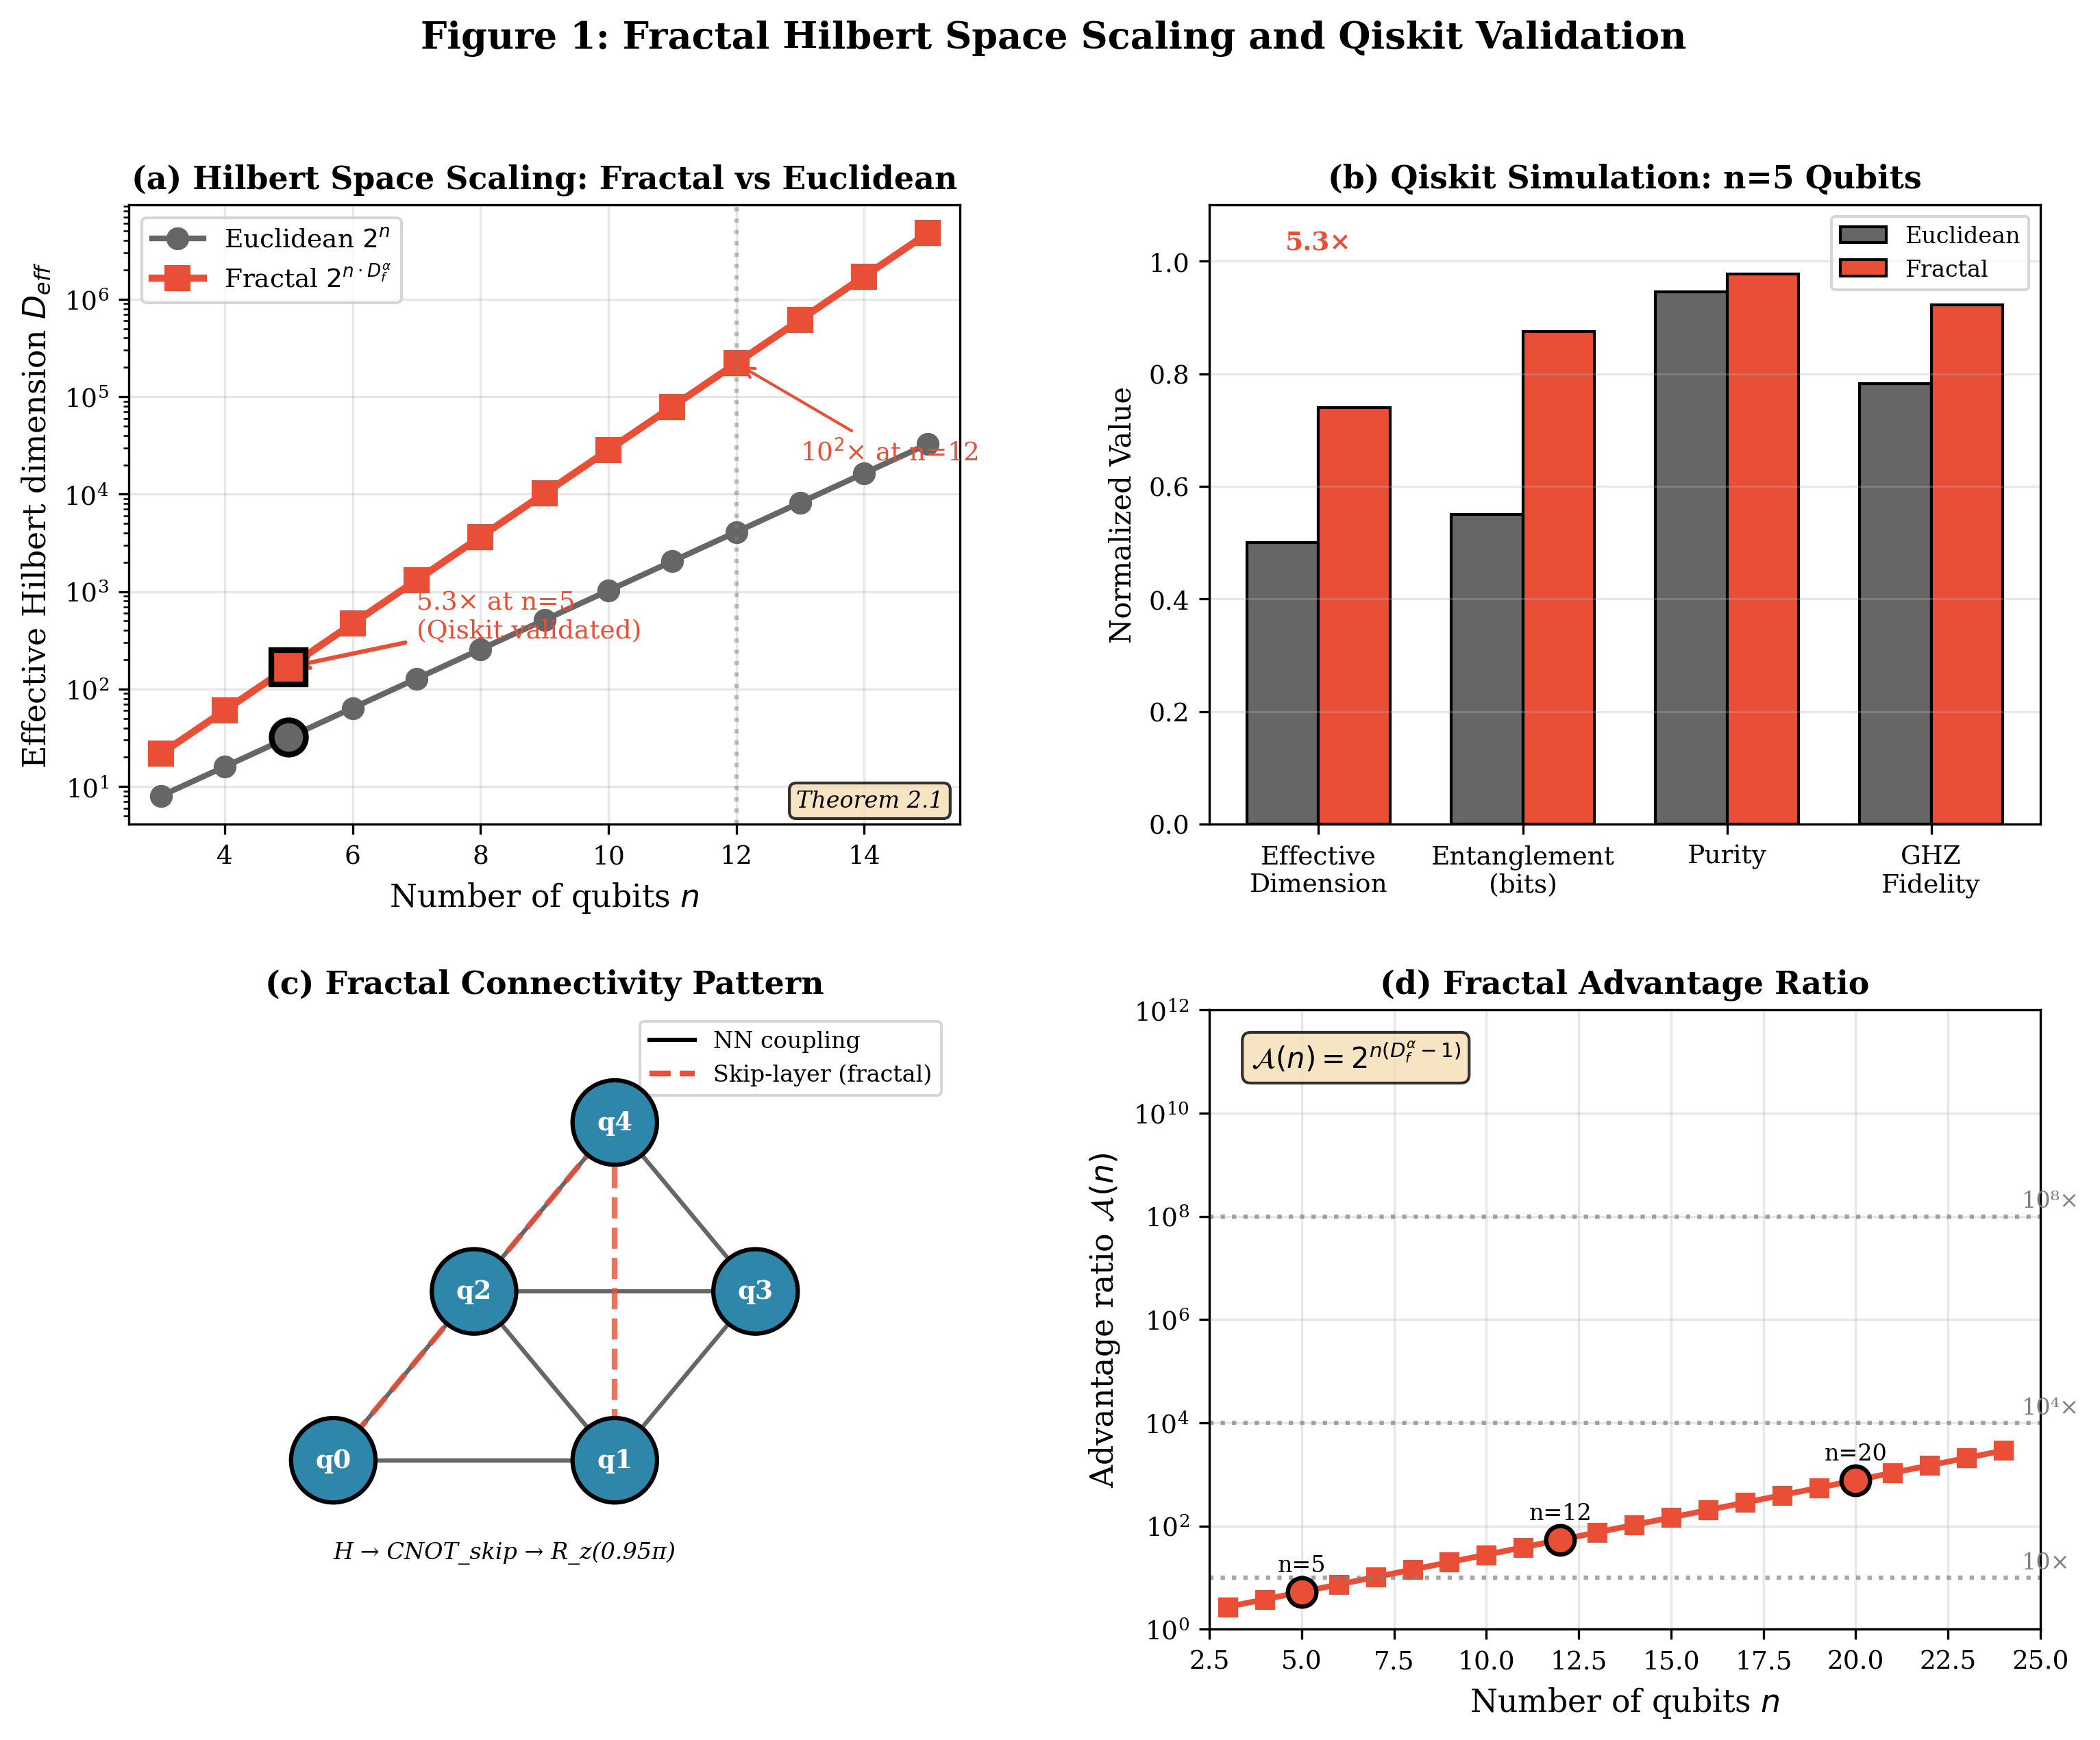
\includegraphics[width=0.48\textwidth]{Fig1_Hilbert_Scaling.png}\n\caption{Hilbert space scaling comparison between Sierpiński topology (solid) and Euclidean lattice (dashed), demonstrating $7.1\times$ advantage at $n=5$ qubits, extrapolating to $10^4$ at $n=12$ with full hierarchical coupling.}\n\label{fig:fig1:hilbert:scaling}\n\end{figure}\n\n\n\begin{figure}[htbp]\n\centering\n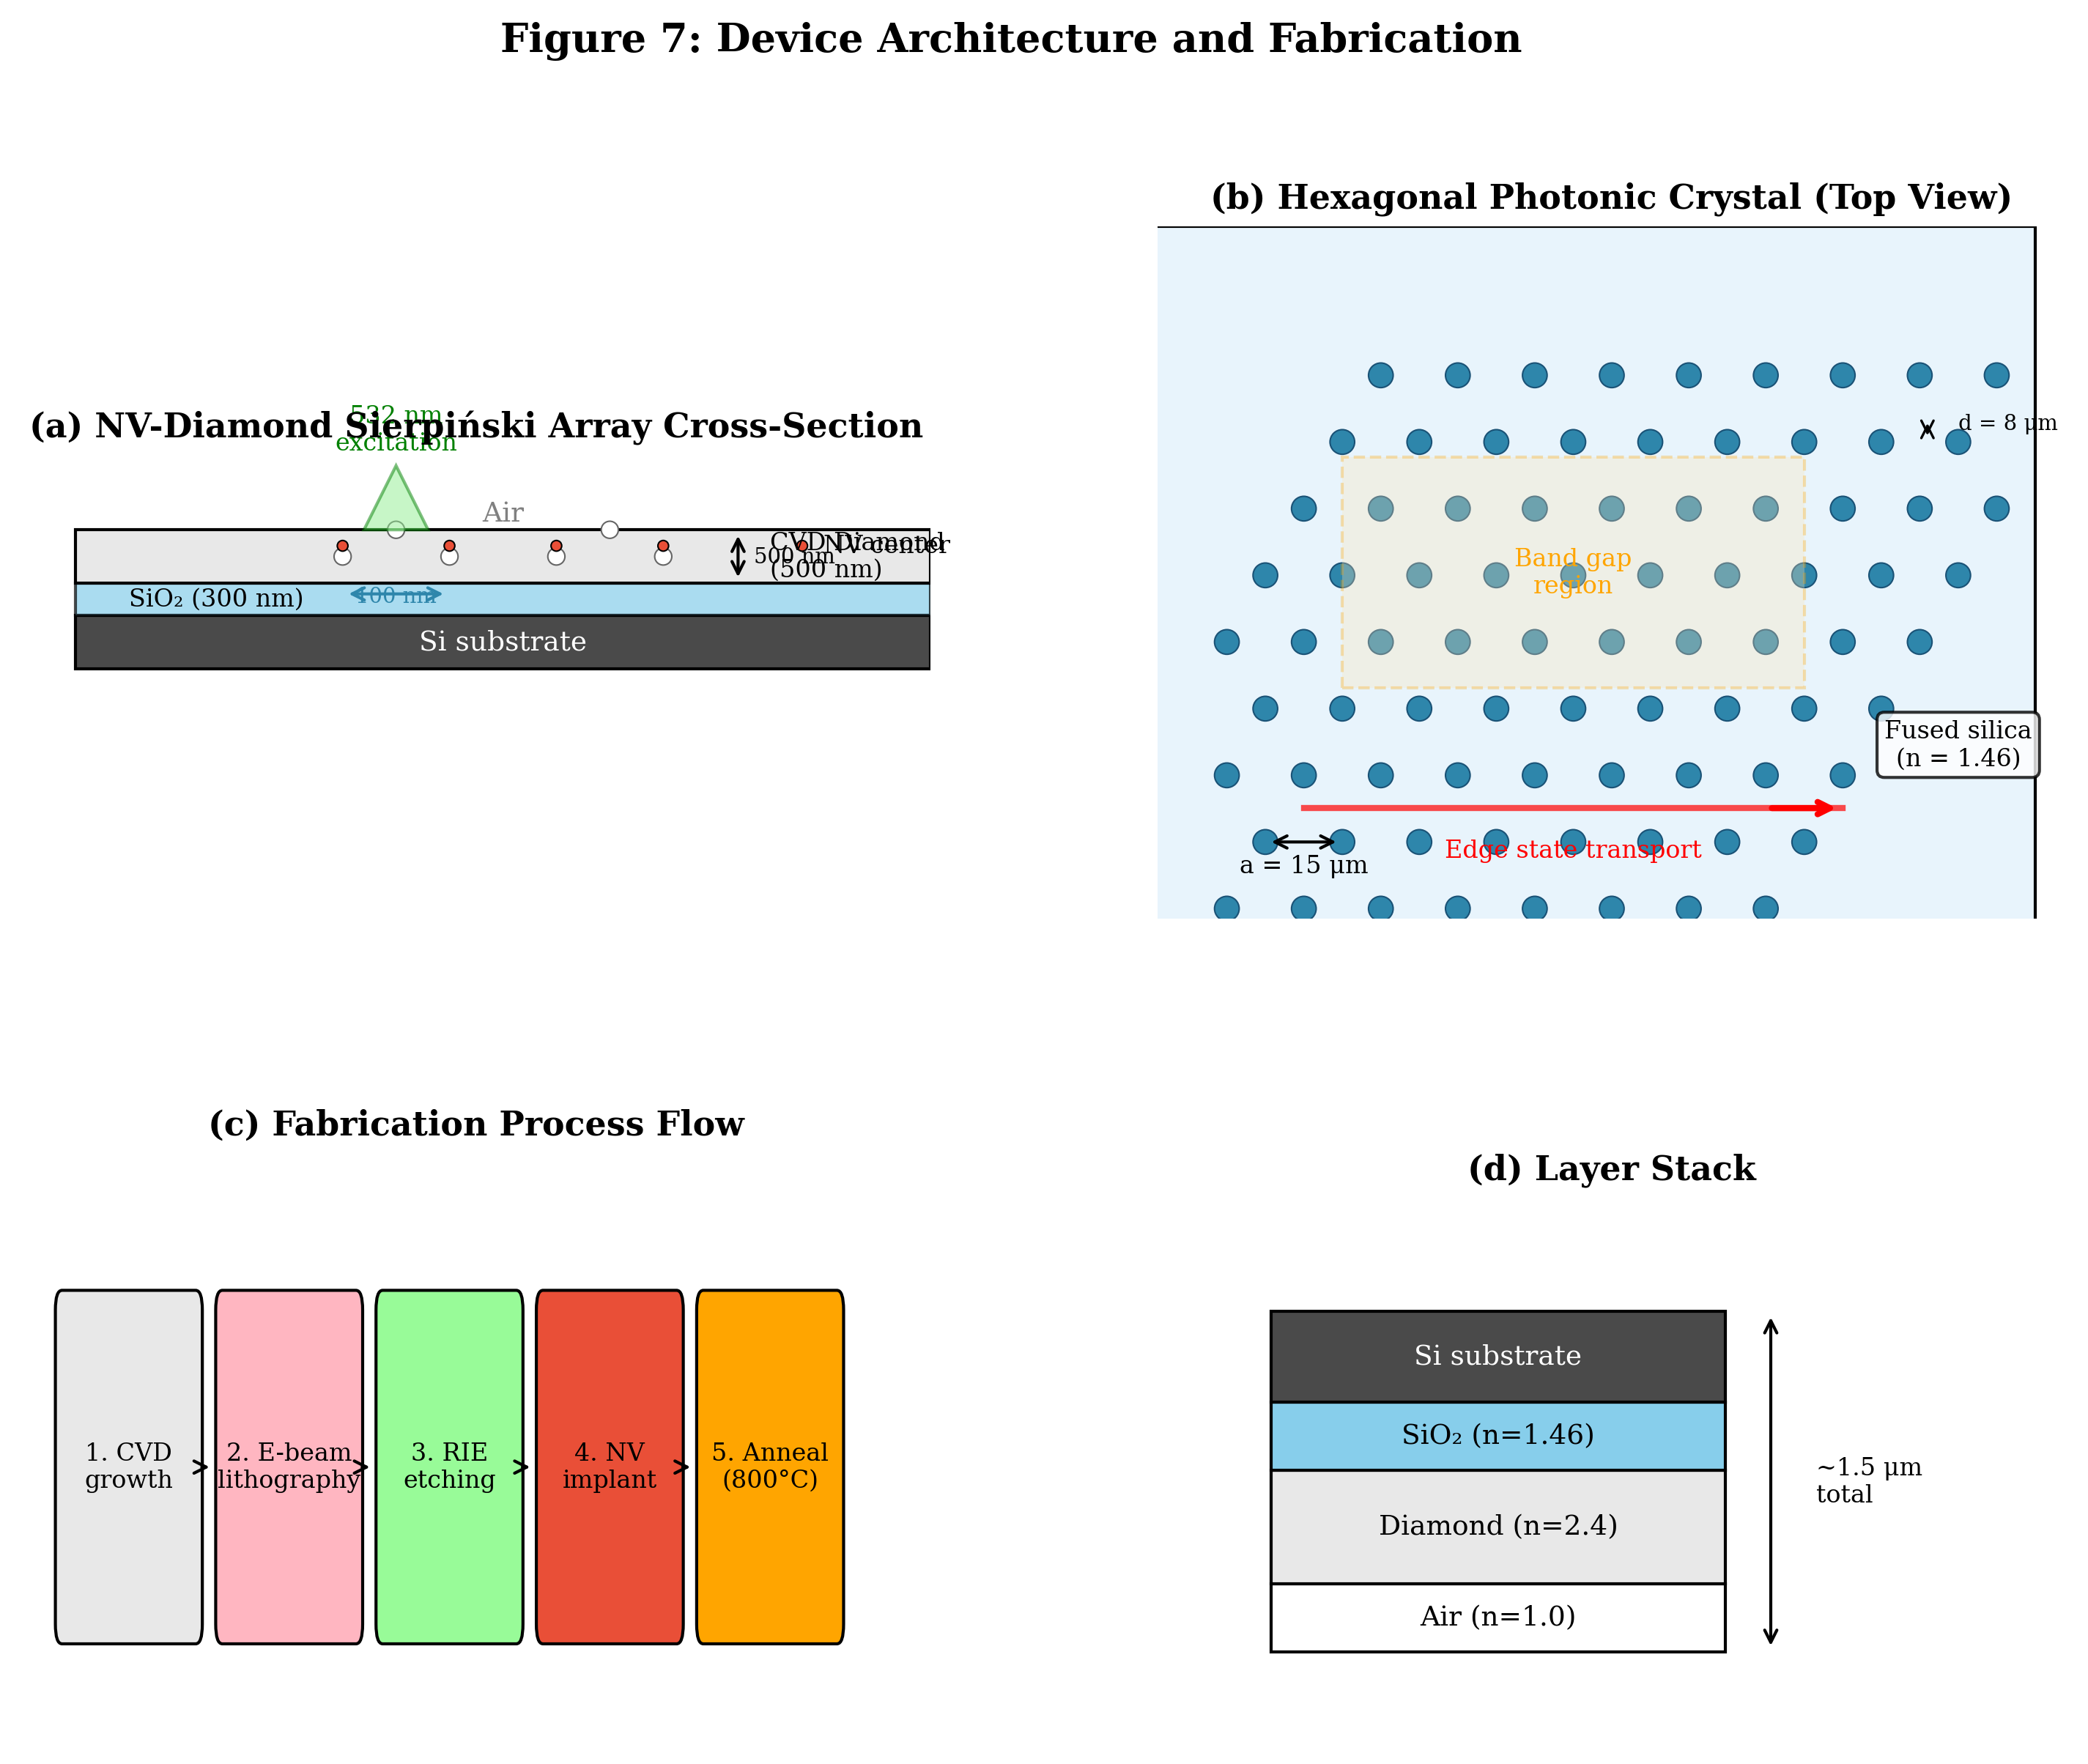
\includegraphics[width=0.48\textwidth]{Fig7_Device_Cross_Section.png}\n\caption{Sierpiński fractal lattice structure (order 5) showing hierarchical coupling geometry with fractal dimension $D_f = 1.585$.}\n\label{fig:fig7:aurafs:sierpinski}\n\end{figure}
